\chapter{A microcell oriented load balancing technique}

In this work, \cite{ahmed2008mol} present a microcell oriented load balancing mechanism in the context of a hybrid MMOG (massively multiplayer online game) architecture. The objective of the proposed approach is to define a fair load balancing model for peer-to-peer MMOGs and virtual environments that minimizes peer-to-peer distortions in the overlays. In the case of an overloaded server, the proposed approach identifies appropriate microcell(s) that reduces overlay maintenance cost and minimizes inter-server communications. The load is relieved by devolving these microcells to the other less loaded servers.



\section{Using microcells}

In this model, a set of microcells defines the virtual game world that is maintained and coordinated by a set of servers called server pool. The server pool having $n$ servers is represented by a set $S = {S_1, S_2, ..., S_n}$. Each server, e.g. $S_i$, serves one or more microcells depending on load distribution and avatars' population in the corresponding microcells. The microcells are given unique identification numbers: left to right, top to bottom in order. In zonal MMOGs, the game world is usually divided into several manageable regions like zones. The zone concept is not entirely new and has been considered over the last few years. The hexagonal shape has a couple of advantages over others like circular, hence considered in this design to define the shape of a microcell. Each microcell is run by a server called master: a special node that coordinates the interactions in a collaborative manner with the active participation of the microcell members, i.e. avatars. So, a set of master nodes, i.e. the server pool, regulates the operation of the MMOG and provides overlay services. In that sense, the system is hybrid as it combines the benefits of both centralized and distributed systems. The layout of microcells and a random microcell distribution to servers are shown in Figure \ref{fig:ahmedmicro}.

\begin{figure}
 \centering
 \includegraphics[width=0.8\textwidth]{images/ahmedmicro}
 \caption{The layout of microcells and a random microcell distribution to servers}
 \label{fig:ahmedmicro}
\end{figure}



\section{Authors' Load definition}

In this work, the authors try to deal with hotspots. So, the implied resolution in this regard is that the server pool can handle the total system load. A hotspot refers to a crowded region in a zonal MMOG, leading to the need for load balancing. But, the key question is how to figure out a hotspot. Most of the approaches consider the total number of players in a zone/microcell as an identifying attribute. If the total number of players in a microcell exceeds the maximum affordable limit, it is a hotspot. Logically, it is correct. But, here the authors look at it in a different way. In MMOGs, there are many players like soldiers, robots, aircrafts, etc. with various features. In addition, the actions that actually take place in a game have an influence on message generation rate. For example, in spite of the regular updates from a player, there may be an immediate message due to a trigger in a pistol by an avatar. Every message requires reaching to every other interested player in the interested region which eventually increases the load of the master. So, the load is not completely related to the number of players, actually, it is purely linked with the message generation rate. Thus, the message generation rate, $R^m$, is used to estimate the load of the masters.



\section{Marking of a loaded server}

Say, the server, $S_i$, is in charge of a set of microcells, $M_i = {m_{i_1} ,m_{i_2} , ..., m_{i_k}}$. Let $R^m_i = {r_{i_1} , r_{i_2} , ..., r_{i_k}}$ are the message generation rate of the microcells ${m_{i_1}, m_{i_2} , ..., m_{i_k}}$ respectively where all of them are governed by server $S_i$. Thus, the load of the server $S_i$ according to message generation rate is $R^m_i = \sum_{j=1}^k r_{i_j}$. Considering the term $T^m$ as a message threshold, a server is loaded or there is a hotspot if $R^m_i > T^m$.



\section{An approach to load balance}

When there is a hotspot, the load of the concerning server is relieved by moving one or more microcells to other less loaded servers. As the movement of microcell introduces complexities, some intelligence is required to identify the best possible set of microcells that need to be moved.

The reduced deployment and maintenance overhead of the hybrid MMOGs (peers or avatars perform some of the message relaying tasks) come at the cost of performance due to peer dynamics. Many techniques have been proposed in literatures such as entity typing and the smart interest driven zone crossing with buffer region to keep the desired level of performance. As it is difficult to predict avatars' movement around a cell boundary (possible frequent in and out movements), it could be effective to share the relevant state information between two adjacent microcells. Instead of sharing the complete state information, a buffer region is defined between two adjacent microcells, as shown in Figure \ref{fig:ahmedbufferregion}. This greatly reduces exchanging of unimportant messages. But, if two adjacent microcells are handled by a single master, there is no buffer region in between, as shown in Figure \ref{fig:ahmedbufferregion}. According to that figure, there is a buffer region between Microcell 2-4 and Microcell 3-3 as they are administered by two different servers but Microcell 2-4 and Microcell 2-3 have a common master and hence no buffer region in between.

\begin{figure}
 \centering
 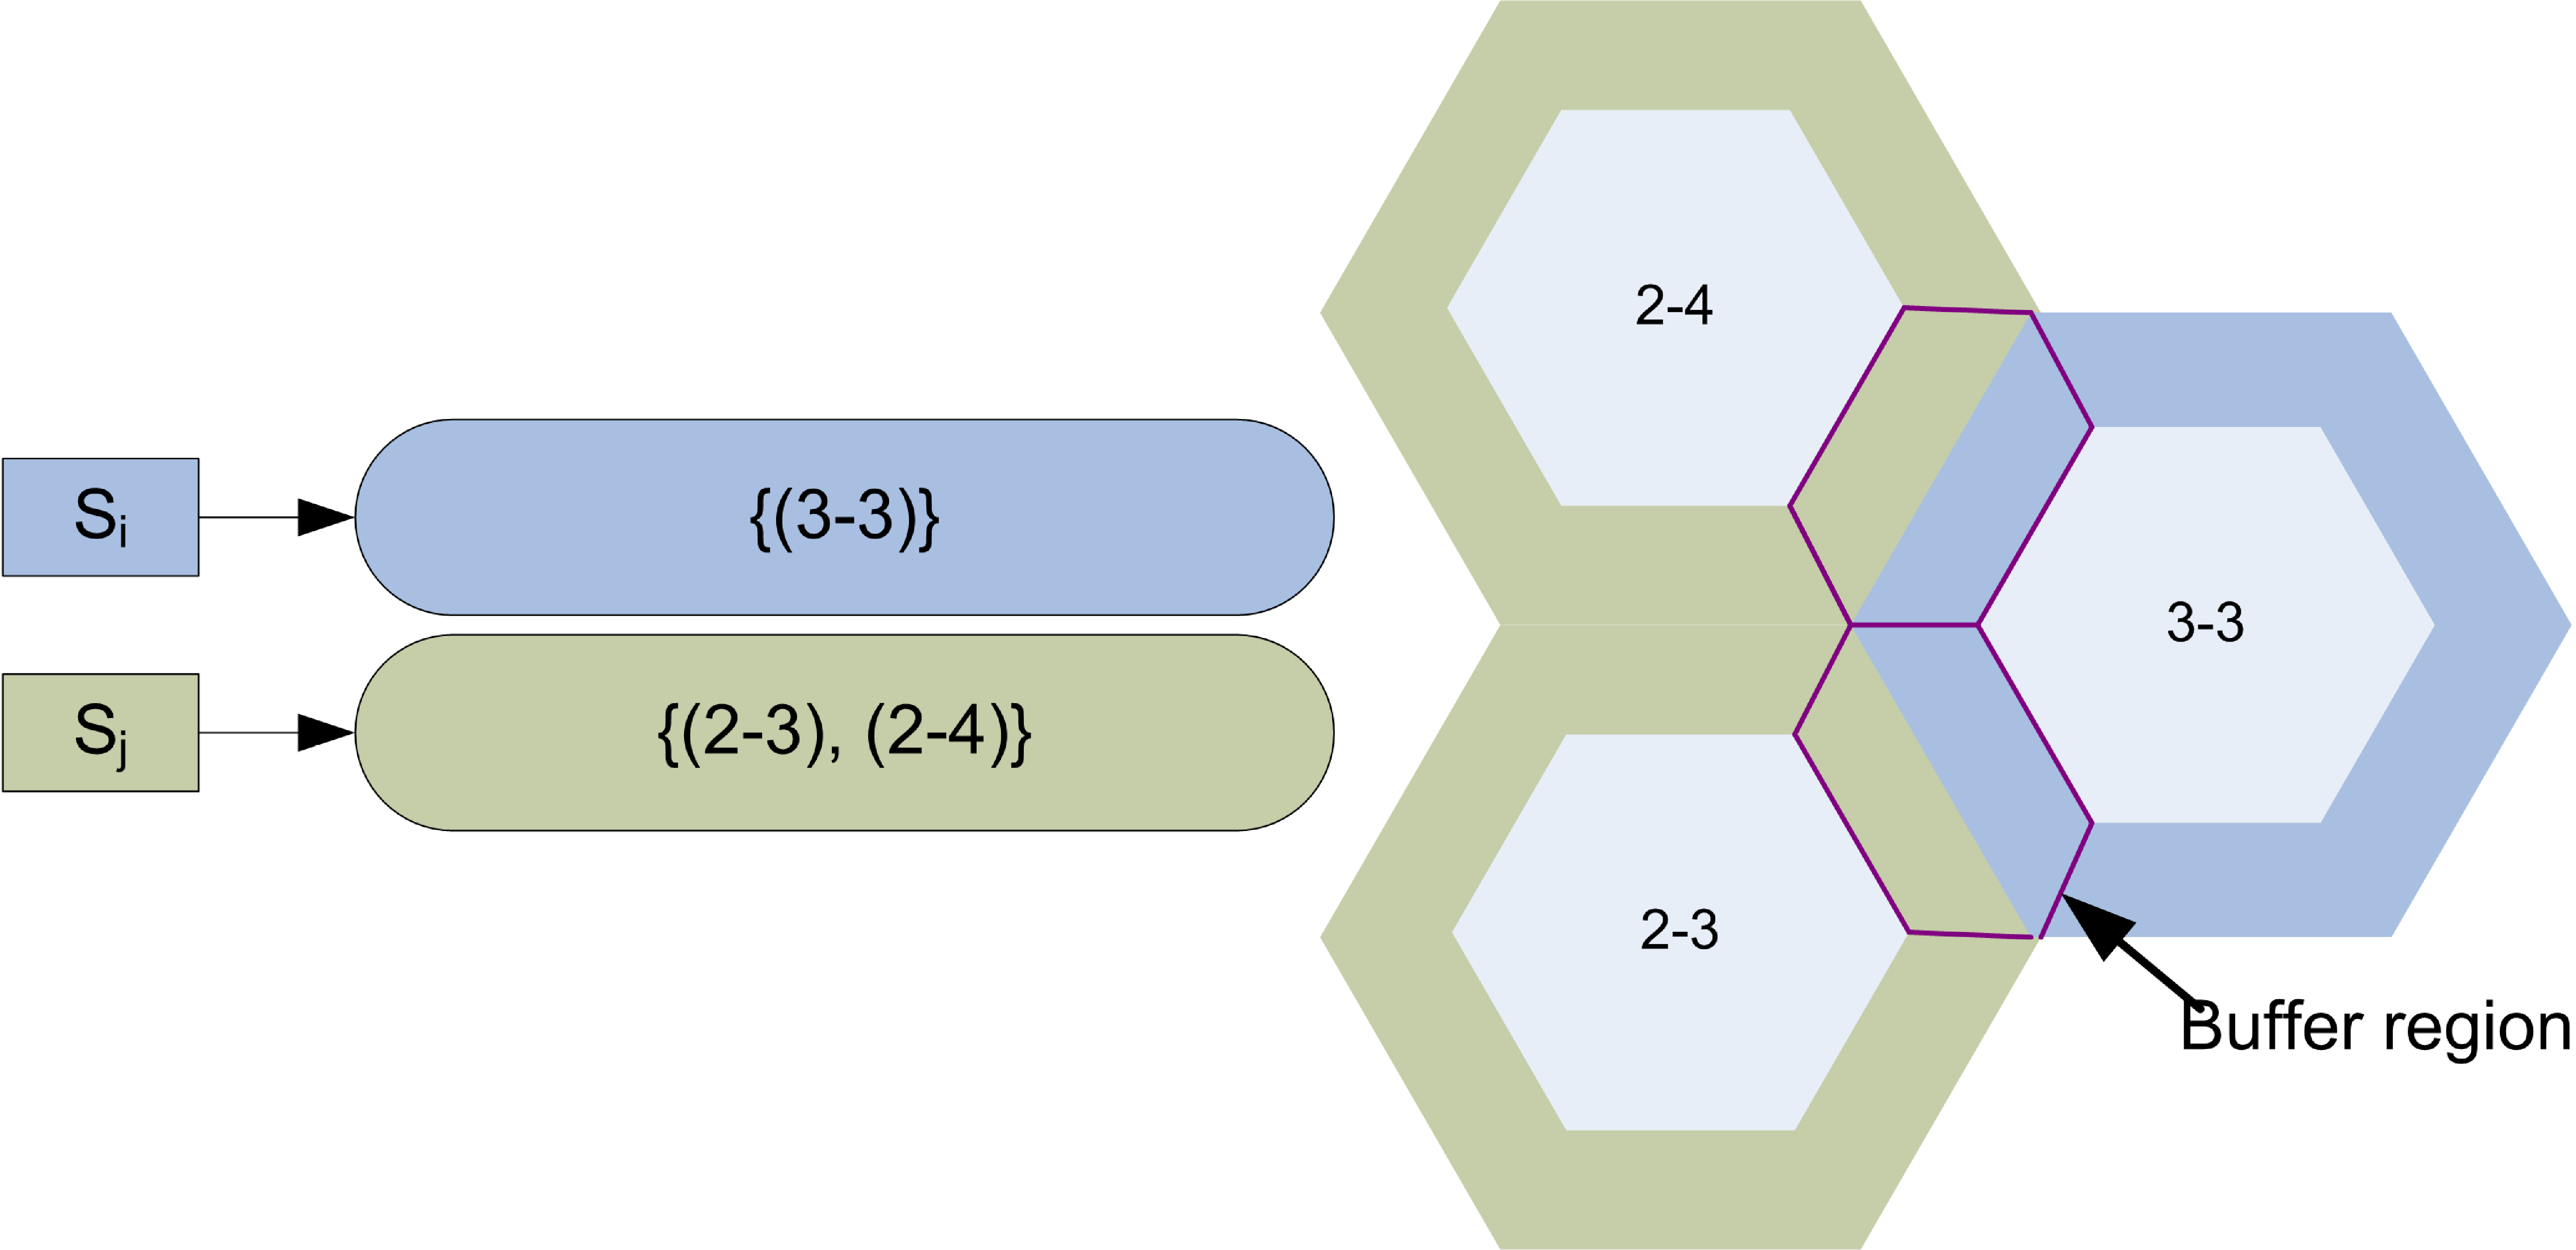
\includegraphics[width=0.8\textwidth]{images/ahmedbufferregion}
 \caption{The buffer region and microcell covering}
 \label{fig:ahmedbufferregion}
\end{figure}

The objective of changing a microcell ownership from one master to another is to approach hotspot. But, the key point that must be taken care of is to minimize inter-server communication cost while carrying out such microcell ownership alteration. Let, $I_i$ is the number of interested links completely internal to the Microcell $i$ among the avatars and $B_{i,j}$ is the number of interested links involved between Microcell $i$ and Microcell $j$ in the buffer region.

Let, the Server $S_i$ is overloaded and currently serving $k$ microcells: $M_i = {m_{i_1} ,m_{i_2} , ..., m_{i_k}}$. The target is to determine an ordered list of microcells so that the microcell ownership alteration according to that order will introduce less performance penalty in the overlays of hybrid MMOGs. The algorithm initially forms group of microcells based on the microcell's neighborhood properties. A microcell can be a member of a nonempty group if and only if it has a common edge with any microcells of that group. Let, after the application of this grouping policy, Server $S_i$ has $l$ groups $G^i_1, G^i_2, ..., G^i_l$ in order of their cardinality, i.e. $|G^i_1| \leq |G^i_2| \leq ... \leq |G^i_l|$. The general strategy is to find a microcell within a group with a minimum number of interested links among the microcells of that group. Due to the change of ownership, these links become foreign links that will cause inter-server communication. Thus, a group with more microcells may have more common edges than a small group, at least heuristically. Thus, it can be effective to keep those groups intact. So, a group with a fewer microcells is chosen for load balancing and that is why we start with the group $G^i_1$, then $G^i_2$ and so on, if necessary. Finally within a group, a microcell with a minimum number of potential foreign links is considered for ownership alteration.



\section{Work analysis}

In this work, \cite{ahmed2008mol} have proposed a microcell oriented load balancing mechanism for peer-to-peer MMOGs. The objective of the proposed approach was to discover one or more microcells of a loaded server in terms of low movement cost. In the case of an overloaded server, the proposed approach identifies microcell(s) that reduces overlay maintenance cost and lowers inter-server communications. The load is reduced by devolving these microcells to the least loaded server.

The problem with this approach, although it considers important aspects of load balancing for MMOGs, is that the server to which the moved microcell is destined is always the least loaded one -- besides the fact that the authors chose to consider a homogeneous server system. By transferring microcells this way between servers, the load balancing scheme induces to regions to become more and more fragmented, which ultimately leads to a higher inter-server communication. This problem, thus, is dealt with by the technique presented in the next chapter.